\paragraph{La classe MainActivity}

\begin{minipage}
    {\linewidth}
    \centering
    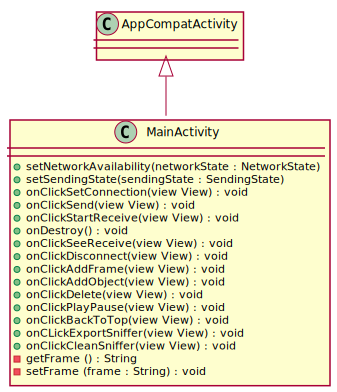
\includegraphics[width=0.60\linewidth]{../schemas/Conception_detaillee/classe_mainActivity.pdf}
    \captionof{figure}{Diagramme de classe de MainActivity}
\end{minipage}

\subparagraph{Philosophie de conception \newline} 

\medspace

La classe MainActivity permet de gérer les interfaces utilisateur de l'application {\nomApplication}. Elle est la classe centrale de l'IHM. 

\subparagraph{Description structurelle \newline}

\medspace

\textbf{Attributs :}

N.A.

\textbf{Services offerts :}

\begin{itemize}
    \item \textbf{setNetworkAvailability(networkState : NetworkState)}  --- Opération qui est appelée lorsqu'on clique sur le bouton de connexion.
    \item \textbf{setSendingState(sendingState : SendingState)}  --- Opération qui permet de mettre à jour l'état d'envoi.
    \item \textbf{onClickSetConnection(view View) : void}  --- Opération qui est appelée lorsqu'on clique sur le bouton de connexion.
    \item \textbf{onClickSend(view View) : void}  --- Opération qui est appelée lorsqu'on clique sur le bouton d'envoi.
    \item \textbf{onClickStartReceive(view View) : void}  --- Opération qui est appelée lorsqu'on clique sur le bouton de réception.
    \item \textbf{onDestroy() : void}  --- Opération qui est appelée lors de la fermeture de l'activité principale. Elle permet la déconnexion. 
    \item \textbf{onClickSeeReceive(view View) : void}  --- Opération qui est appelée lorsqu'on clique sur le bouton d'affichage de la réception.
    \item \textbf{onClickDisconnect(view View) : void}  --- Opération qui est appelée lorsqu'on clique sur le bouton de déconnexion.
    \item \textbf{onClickAddFrame(view View) : void}  --- Opération qui est appelée lors de l'ajout d'une trame dans un objet, par un clique sur le bouton [ajouterTrame].
    \item \textbf{onClickAddObject(view View) : void}  --- Opération qui est appelée lors de l'ajout d'un objet, par un clique sur le bouton [ajouterObjet].
    \item \textbf{onClickDelete(view View) : void}  --- Opération qui est appelée lors de la suppression d'un ou plusieurs éléments. 
    \item \textbf{onClickPlayPause(view View) : void}  --- Opération qui est appelée lors de la mise en pause/play du sniffer. 
    \item \textbf{onClickBackToTop(view View) : void}  --- Opération qui est appelée lorsque Utilisateur souhaite revenir en haut du sniffer.
    \item \textbf{onCLickExportSniffer(view View) : void}  --- Opération qui est appelée lors de l'export du sniffer. 
    \item \textbf{onClickCleanSniffer(view View) : void}  --- Opération qui est appelée lors d'un clique sur le bouton [viderSniffer], c'est à dire, de manière à vider le sniffer des trames actuelles.
    \item \textbf{getFrame () : String}  --- Opération qui est appelée lorsqu'on souhaite récupérer la dernière trame reçue.
    \item \textbf{setFrame (frame : String) : void}  --- Opération qui permet de mettre à jour la dernière trame reçue. 
   
\end{itemize}
